\documentclass[12pt]{article}

\usepackage{amsfonts}
\usepackage{graphicx}
\usepackage[all]{xy}
\usepackage{amsthm}
\usepackage{amsmath}
\usepackage{tikz,lipsum,lmodern}
\usepackage[most]{tcolorbox}
\usepackage{makeidx}
\usepackage[pdftex]{hyperref}
\usepackage{color, colortbl}
\usepackage{amssymb}
\usepackage{mathrsfs}
\usepackage{longtable}
\usepackage{wasysym}
\usepackage{float}   

\theoremstyle{definition} \newtheorem{prob}{Problem}
\theoremstyle{definition} \newtheorem{cprob}{Challenge Problem}
\theoremstyle{definition} \newtheorem{sol}{Solution}
\newtheorem*{thm}{Theorem}
\newtheorem*{lem}{Lemma}
\newtheorem*{prop}{Proposition}

% Add a period after the section number:
\renewcommand\thesection{\arabic{section}.}

\begin{document}

%%%%%%

% NOTE: To turn this into a solution set, use %'s to comment out the material
% just above this line, and remove the %'s to use the material just below it
% as the heading for your document.

\begin{center}
  Will Drake
\end{center}

\begin{center}
  \rule{10cm}{0.1pt}
\end{center}

\section{Introduction}
The game I chose to model was a tile slider puzzle.
As a kid, I had my own small slider puzzle (Figure 1). I was thus motivated to create a game similar to this.

\begin{figure}[H]
  \centering
  \caption{}
  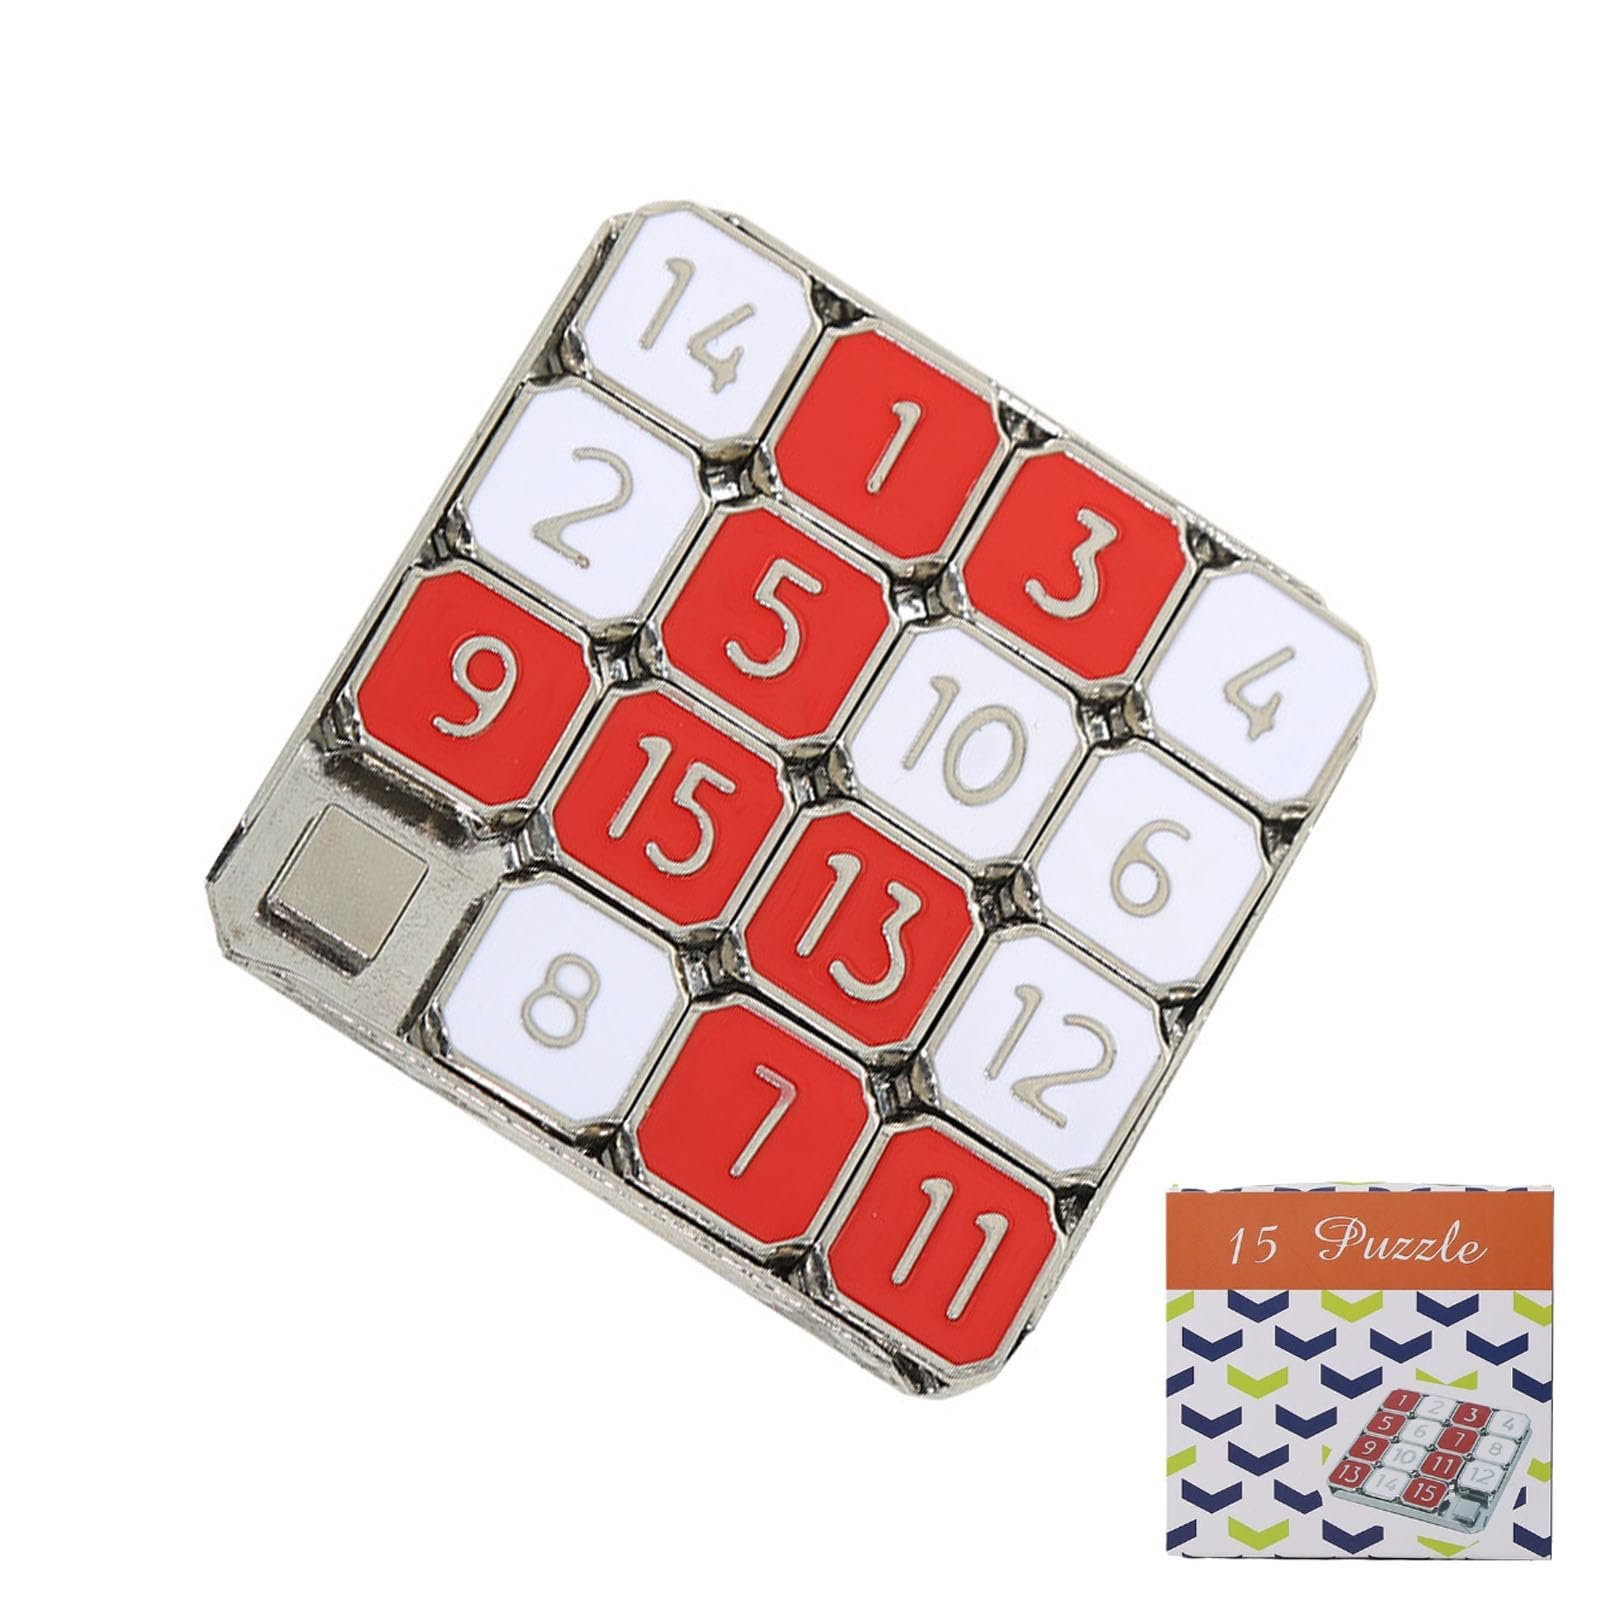
\includegraphics[width=0.6\textwidth]{download.jpg}
  \label{fig:slider-puzzle}
\end{figure}

Since I am very familiar with this puzzle, I wanted to model it and find the minimal solution for a specific randomized starting board. The game works as follows: There is a blank space that allows the player to move tiles. The goal is to take the randomized board and, by sliding numbered tile pieces around, get them in order from left to right, with the blank being in the bottom right.

\section{Code, Formalization, and Analysis}
For my tile game, I did a $3\times 3$ to save monotonous writing of more tiles and a large number of moves or boards that would take a while to compile. However, since the fundamental moves for the tile game are the same, this code can be easily adapted to $4\times 4$, $5\times 5$ or beyond by simply changing the board and adding more tiles. For the code in Alloy, I started by using the tic tac toe model we did in class and adapted the code to work for my tile game. Similarly to tic tac toe, this tile game would be a $3\times 3$ using row and columns; however, I also needed to map each row and col to a single tile. Thus, giving me my \texttt{sig Board} adapted from tic tac toe to be
\[
  \mathrm{Row} \;\to\; \mathrm{Col} \;\to\; \text{one Tile}.
\]
With my board ready, I created two predicates, one with the randomized \texttt{StartingBoard} and one with the \texttt{EndingBoard}; these would serve to work with my movement of the game to have a start and end. The movement of the game was the most challenging part and required the most thought. When you are playing the game in real life, you think of the movement as sliding a piece into an open space. To formalize this in Alloy, I needed to decide how movement could properly work for an Alloy implementation. Instead of thinking of it as sliding pieces, I thought of the blank space and a tile switching row and column positions. This can happen for any piece that is to the left, right, up, or down of the blank space.

I started by creating a \texttt{Neighbors} predicate, allowing me to identify the pieces that are on the left, right, up or down. For left and right pieces, the row would stay the same but the column would either be plus one or minus one, giving me the code.

\[
  (\,i_1 = i_2 \;\wedge\; (\,j_2 = \mathrm{add}[\,j_1,1\,]\;\vee\; j_2 = \mathrm{sub}[\,j_1,1\,]\,)).
\]

For up and down the column would stay the same but the row would either be plus one or minus one, thus

\[
  (\,j_1 = j_2 \;\wedge\; (\,i_2 = \mathrm{add}[\,i_1,1\,]\;\vee\; i_2 = \mathrm{sub}[\,i_1,1\,]\,)).
\]

Combining these with $\vee$ gives me all the neighbors possible. Next, I moved on to the \texttt{LegalMove} predicate. Having some \texttt{tile1} and some \texttt{tile2} with their respective row and col, I would have \texttt{tile1} be equal to the \texttt{Blank} and \texttt{tile2} be a neighbor of \texttt{tile1} for \texttt{board1}. 
Then I would set the \texttt{Blank} equal to the neighbor for \texttt{board2} and vice versa:
\begin{align*}
  \text{some } &i_1:\mathrm{Row},\,i_2:\mathrm{Row},\,j_1:\mathrm{Col},\,j_2:\mathrm{Col}\;\big|\;
    b_1.\mathrm{at}[i_1,j_1] = \mathrm{Blank}
    \;\wedge\;
    \mathrm{Neighbors}[\,i_1,j_1,i_2,j_2\,]\\
  &\wedge\;
    b_2.\mathrm{at}[i_1,j_1] = b_1.\mathrm{at}[i_2,j_2]
    \;\wedge\;
    b_2.\mathrm{at}[i_2,j_2] = \mathrm{Blank}.
\end{align*}

Although this movement works perfectly, I need to ensure that no other tiles would change positions besides the blank and its neighbor, so I enforced that for all rows and columns, if they were not these two tiles, their position in \texttt{board1} and \texttt{board2} would be the same. So I added this onto \texttt{LegalMove}:

\begin{align*}
  \text{all } &r:\mathrm{Row},\,c:\mathrm{Col}\;|\;\neg\bigl((r\!\to\!c)\in (\,i_1\!\to\!j_1)\,\cup\,(i_2\!\to\!j_2)\bigr)\\
  &\qquad\implies b_2.\mathrm{at}[r,c] = b_1.\mathrm{at}[r,c].
\end{align*}

With all this working I took the \texttt{Game} predicate with my \texttt{StartingBoard}, then applied \texttt{LegalMove} one board after another, ending with my \texttt{EndingBoard}. Through checking the game with different number of Boards, I discovered the \texttt{MinimalSolution} for my specific randomized tile slider was 23 moves.



\section{Further Work}
The next step with this game would be to look at different variations. The slider puzzle is always a square with the same amount of rows and columns, but what about looking at sliders with different amount of rows and columns? Are they still solvable in every state? If not, how many states are they solvable in? Are they solvable at all?

\end{document}
\begin{figure}
    \centering
    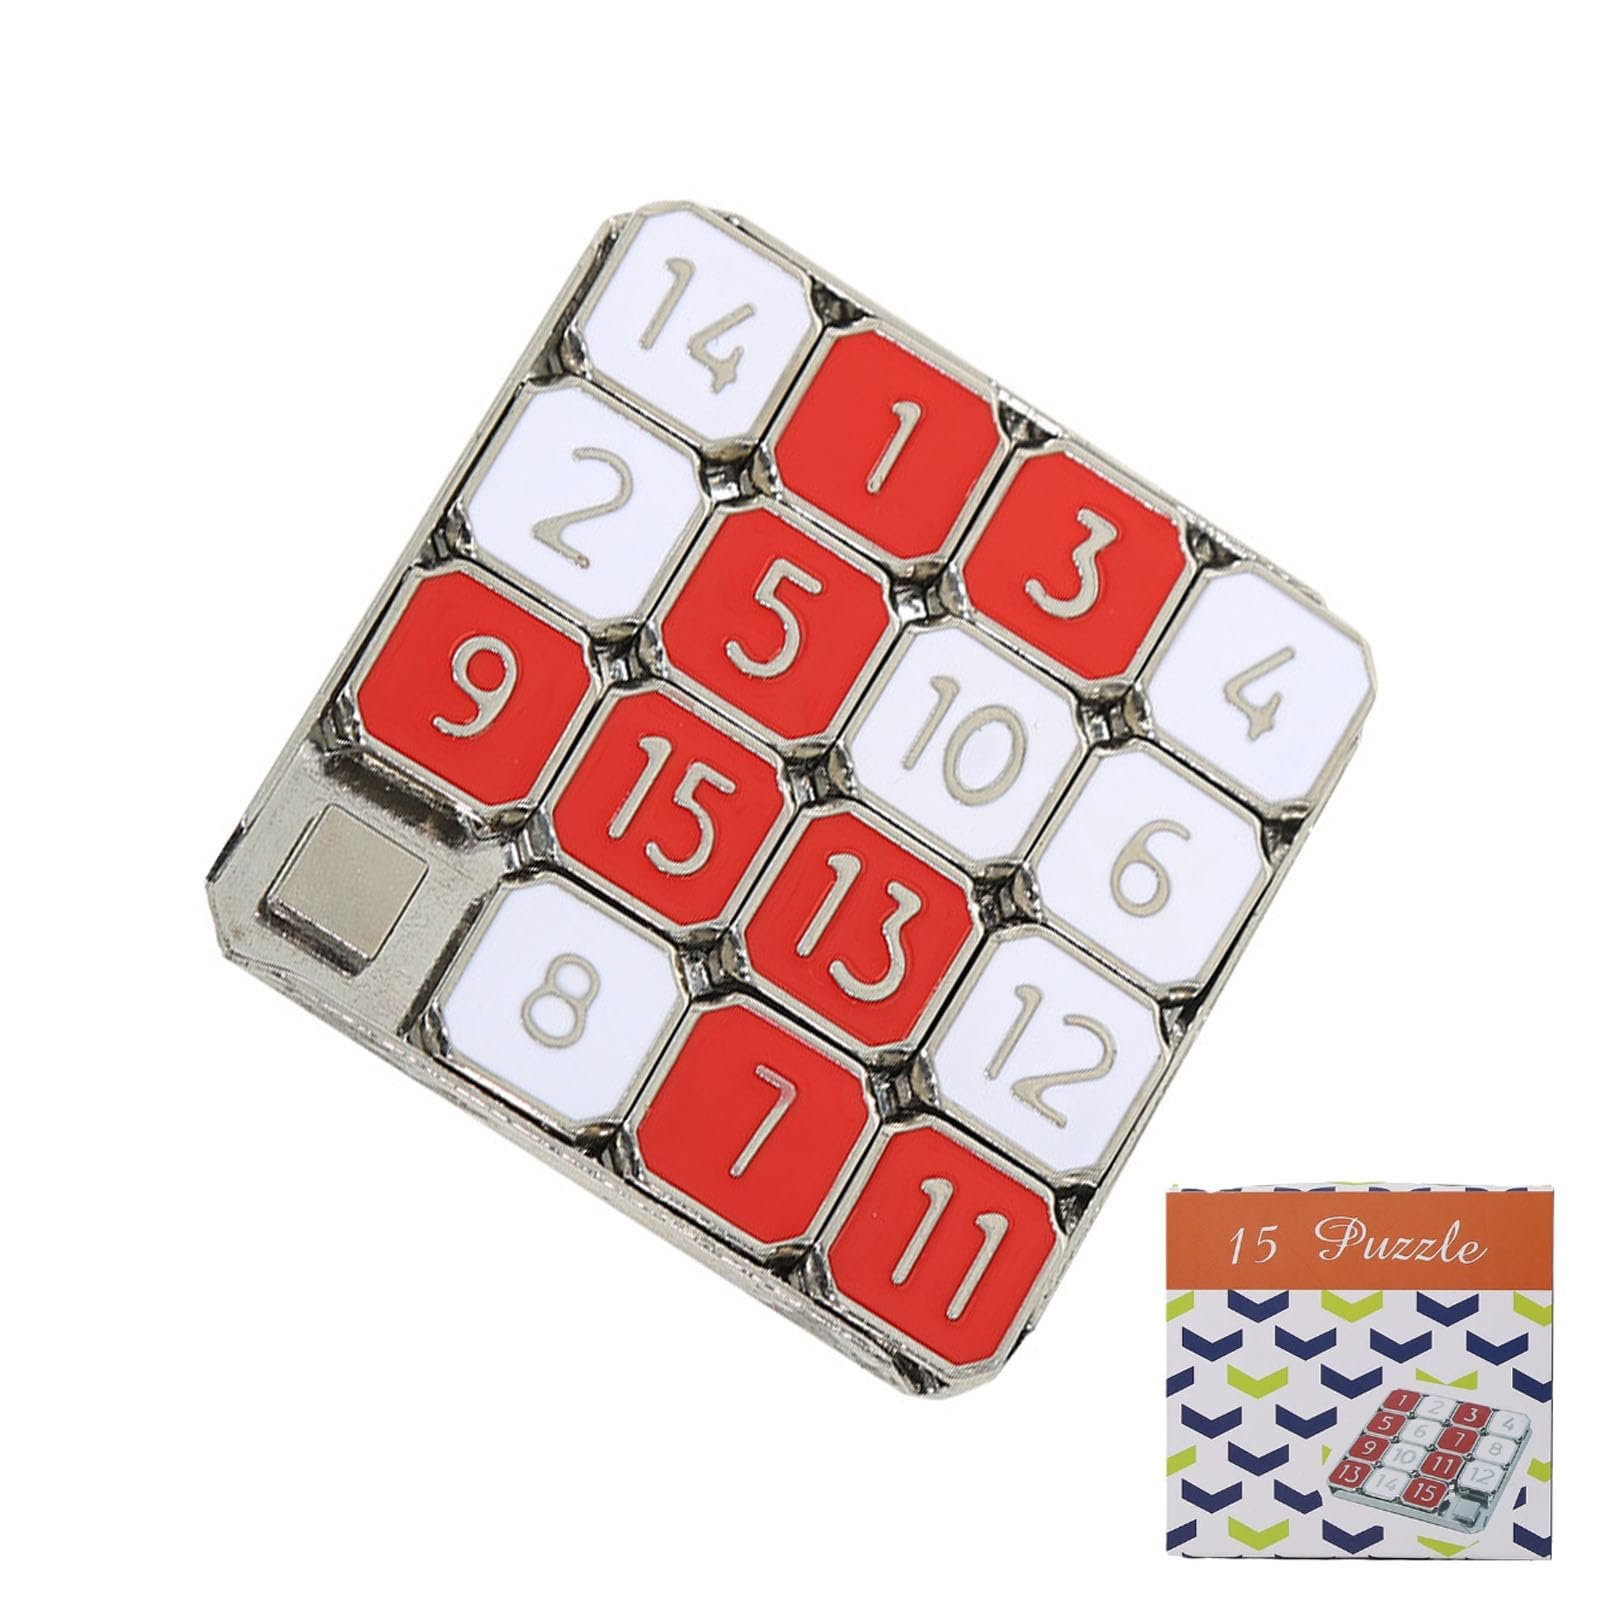
\includegraphics[width=0.5\linewidth]{download.jpg}
    \caption{Enter Caption}
    \label{fig:enter-label}
\end{figure}
